


%\bf{摘要:} 本文提出一种

%\noindent 中文字体(默认宋体)\\
%\fangsong 中文字体(仿宋) \songti 中文字体(宋体) \lishu 中文字体(隶书) \heiti 中文字体(黑体)\\
%\CJKfamily{zhkai} 中文字体(楷书) \CJKfamily{zhyou} 中文字体(幼圆) \CJKfamily{zhyahei} 中文字体(微软雅黑)\\


%\textbf{摘要:}中文摘要中文摘要中文摘要中文摘要中文摘要中文摘要中文摘要中文摘要中文摘要中文摘要中文摘要中文摘要
%
%\textbf{关键词:}关键词1;关键词2;关键词3。

% \textbf{Abstract:} AbstractAbstractAbstractAbstractAbstractAbstractAbstractAbstractAbstractAbstractAbstractAbstractAbstractAbstractAbstract.

% \textbf{keywords: }keywords, keywords, keywords, keywords.
%\setlength{\parindent}{2em} 

%\section{前言}
%
%\label{intro}
%前言前言前言前言前言前言前言前言前言前言前言前言前言前言
%
%前言前言前言前言前言前言前言前言前言前言前言前言前言前言
%
%前言前言前言前言前言前言前言前言前言前言前言前言前言前言
%
%前言前言前言前言前言前言前言前言前言前言前言前言前言前言
%
%前言前言前言前言前言前言前言前言前言前言前言前言前言前言
%
%前言前言前言前言前言前言前言前言前言前言前言前言前言前言
%
%前言前言前言前言前言前言前言前言前言前言前言前言前言前言
%
%前言前言前言前言前言前言前言前言前言前言前言前言前言前言
%
%前言前言前言前言前言前言前言前言前言前言前言前言前言前言
%
%前言前言前言前言前言前言前言前言前言前言前言前言前言前言
%
%
%\begin{figure}[!h]
%	\centering
%	\includegraphics{Fig/Fig1.eps}
%	\caption{无人机}
%	\label{fig:1}     
%\end{figure}

% \textbf{\fangsong\xiaosihao 二、立题依据}
% \vspace{-0.30cm}
\begin{ubox}
	\setlength{\parindent}{0em} 
开题以来研究工作总结:
\vspace{-0.25cm}

% 2、国内外研究现状(工程应用现状)
% \vspace{-0.25cm}

% 3、主要参考文献及出处
\setlength{\parindent}{2em} 

目前涵道式无人机的相关研究主要集中在平稳飞行控制,针对高机动飞行时存在系统模型气动机理复杂、不确定性高、易受干扰等问题。自开题以来进展包括:

1)xx姿态控制策略。

2)将第一项工作的内容抽象出其数学本质。



3)针对机动飞行过程的动态问题,尝试建立动态过渡走廊的一般性描述与构建方法。



下面对上述三项研究进展分别阐述。

\textbf{\fangsong\xiaosihao 一、姿态控制策略}
\setlength{\parindent}{2em} 
% \section{前言}
% \label{intro}

在本项工作中,我们提出了一种使用xx的模块化角速度控制器设计。 通过引入xx. 该项工作的主要贡献总结如下:
\begin{figure}[H]
	\centering
	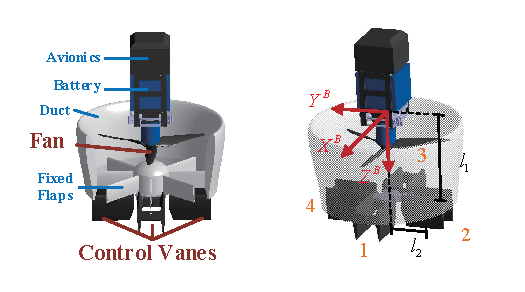
\includegraphics{Fig/Fig2.eps}
	\caption{涵道风扇无人机布局}
	\label{fig:2}     
\end{figure}
1). 首次。

2). 针对。

3). 所提出的进行了试验验证。

\section{建模}
\label{sec:1}
如图\ref{fig:2}所示,本文所研究的涵道风扇无人机配置有一个风扇和四个交叉布置的控制舵。 为了平衡风扇扭矩,固定气动襟翼放置在控制舵上方,涵道气流将对这些襟翼产生反扭矩作用。 与多旋翼不同,控制舵产生的力矩不是由舵偏转角独立决定的,而是与涵道流出速度相结合,显示出推力矢量特性。 但在大多数涵道风扇控制案例中,风扇只是通过控制转速来产生推力,飞行器的姿态完全由舵偏转角控制。


\subsection{符号约定}
涵道风扇无人机的机体系如图 \ref{fig:2} 所示。 机体系的原点位于重心,正交的机体轴线表示为$\text{ }\!\!\{\!\!\text{ }{\bm{X}^{B}},{\bm{Y}^{B}},{\bm{Z}^{B}}\text{ }\!\!\}\!\!\text{ }$。 无人机沿机身轴线的角速度表示为${{\bm{\omega }}^{B}}=[p \quad q \quad r]^{T}$。风扇的转速记为$\Omega$。 每个控制舵的偏转角表示为 ${{\delta }_{i}}$,以矢量形式描述为$[{{\delta }_{1}} \quad {{\delta }_{2}} \quad {{\delta }_{3}} \quad {{\delta }_{4}}]^T$。



惯性系中的速度、惯性系中的姿态和风速分别表示为${{\bm{V}}^{I}}$、$\bm{\eta }$ 和 ${{\bm{W}}^{I}}$。 虽然不涉及角度控制设计,但这里也使用了这些与惯性系相关的变量,因为它们对于指定 INDI 的有效性至关重要。

由于涵道风扇无人机对所有机身轴对称,无人机的惯性矩阵可以简化为对角矩阵,表示为 $ \bm{I}=\text{diag}({{I}_{x} },{{I}_{y}},{{I}_{z}}) $。

在机体坐标系中表示的合力矩表示为 $\bm M$ ,为以下几项的和:
\begin{equation}
	{\bm{M}} = {{\bm{M}}_{vane}} + {{\bm{M}}_{flap}} + {{\bm{M}}_{fan}} + {{\bm{M}}_{aero}}
	\label{eq_1}
\end{equation}
其中 $ {{\bm{M}}_{vane}} $ 是从控制舵产生的控制力矩矢量。 $ {{\bm{M}}_{flap}} $ 是作用在固定气动襟翼上的反扭矩作用。 $ {{\bm{M}}_{fan}}$ 包括来自旋转的风扇的气动扭矩、角加速度力矩和陀螺效应。 $ {{\bm{M}}_{aero}} $ 是气动力矩。

\subsection{控制力矩}
在INDI设计中,只需要辨识控制力矩,控制力矩 ${{\bm{M}}_{vane}} $ 是涵道风扇无人机角速度子系统的控制输入,由控制舵产生。 一个偏转舵受到垂直于无人机 ${{\bm{Z}}^{B}}$ 轴的力,并同时受到两个相对于相应机体系轴的正交力矩。 四个控制舵的总控制力矩可以通过以下公式表示:
\begin{equation}
{{\bm{M}}_{vane}} = {k_{cv}}V_e^2\left[ {\begin{array}{*{20}{c}}
	{{\rm{ - }}{l_1}}&0&{{l_1}}&0\\
	0&{{\rm{ - }}{l_1}}&0&{{l_1}}\\
	{{l_2}}&{{l_2}}&{{l_2}}&{{l_2}}
	\end{array}} \right]{\bm{\delta }}
\label{eq_2}
\end{equation}
其中 $ {{k}_{cv}} $ 是与舵形状相关的常数系数。 $ {{l}_{1}} $ 和 $ {{l}_{2}} $ 是图 \ref{fig:2} 中所示的杠杆臂。 ${{V}_{e}}$ 表示涵道流出的速度,由下式给出:
\begin{equation}
	{V_e} = {k_v}\Omega 
	\label{eq_3}
\end{equation}
其中 $ {{k}_{v}} $ 是与涵道的所有空气动力学特征相结合的常系数。 

如果所有舵偏转角都保持在气动失速极限内,则式 \eqref{eq_2} 中的比例关系成立,表示为 $ {{\delta }_{m}} $。 这是 ${\bm \delta}$ 的基本约束:
\begin{equation} 
	- {\delta _m} \le {\delta _i} \le {\delta _m},   i = 1,2,3,4.
	\label{eq_4}
\end{equation}

显然,式\eqref{eq_2} 将冗余舵偏转角映射到三维的控制力矩,表明无人机角速度子系统的过度驱动特性。 通过使用虚拟控制输入$ \bm{\nu }=[{\nu }_{x} \quad {\nu }_{y} \quad {\nu }_{z}]^{T}$,可以将控制力矩效应重构为模块化形式:
\begin{equation}
	\left\{ \begin{array}{l}
	{{\bm{I}}^{ - 1}}{{\bm{M}}_{vane}} = {{\bm{H}}_1}{\bm{\nu }}{\Omega ^2}\\
	{\bm{\nu }} = {\bm{B\delta }}
	\end{array} \right.
	\label{eq_5}
	\end{equation}
其中
	\begin{equation}
	\begin{array}{ccccc}
	{{\bm{H}}_1} \buildrel \Delta \over =   {k_{cv}}k_v^2\left[ {\begin{array}{*{20}{c}}
		{2I_x^{ - 1}{l_1}}&{}&{}\\
		{}&{2I_y^{ - 1}{l_1}}&{}\\
		{}&{}&{4I_z^{ - 1}{l_2}}
		\end{array}} \right]     \quad
	{\bm{B}} \buildrel \Delta \over =   \left[ {\begin{array}{*{20}{c}}
		{ - 0.5}&0&{0.5}&0\\
		0&{ - 0.5}&0&{0.5}\\
		{0.25}&{0.25}&{0.25}&{0.25}
		\end{array}} \right]
	\end{array}
	\label{eq_6}
\end{equation}

从式 \eqref{eq_5} 和式 \eqref{eq_6} 中,$\bm{B}$ 的定义表示虚拟输入的大小被标准化为 $[-1,1] \centerdot {{\delta }_{m }}$。 通过这种模块化,在式 \eqref{eq_2} 中从舵偏转角到控制力矩的直接映射被转换为从舵偏转角到虚拟输入的映射,而映射矩阵 $\bm{B}$ 不包含模型信息。


\subsection{角速度环动力学}
在无人机控制的意义上,旋转风扇通常被假设为一个圆盘,对飞行器施加稳定的推力和扭矩,因此无人机可以被视为刚体。 因此角速度动力学方程为:
\begin{equation}
	{{\bm{\dot \omega }}^B} = {{\bm{I}}^{ - 1}}\left( {{\bm{M + I}}{{\bm{\omega }}^B}{\bm{ \times }}{{\bm{\omega }}^B}} \right)
	\label{eq_16}
\end{equation}
其中 $\bm M$ 由式 \eqref{eq_1} 预先定义,$\times$ 表示向量的叉积。

\section{控制器设计}
值得注意的是,矩阵 ${{\bm{H}}_{1}}$、${{\bm{H}}_{2}}$ 和 ${{\bm{H}}_{3}}$现在是方阵且可逆。 在上层设计中,我们可以直接在这个模型上应用INDI,而不考虑控制分配问题。


\subsection{控制分配}
在底层设计中,我们解决控制分配问题,即利用下式,对给定的 ${{\bm{\nu }}_{d}}$ 求解适当的舵偏转角 $\bm{\delta }$,
\begin{equation}
	{\bm {\nu}_d}={\bm{B\delta}}
	\label{eq_29.5}
\end{equation}
上式的解表示为 $\bm{\delta }_d$。 具体可以描述为:对于给定的${{\bm{\nu }}_{d}}$,求${{\bm{\delta }}_{d}}\in \Delta $使得 ${{\bm{\nu }}_{d}}=\bm{B}{{\bm{\delta }}_{d}}$,或者最小化分配误差 ${{\bm{\ nu }}_{d}}-\bm{B}{{\bm{\delta }}_{d}}$,其中 $\Delta $ 是允许控制集,定义为:
\begin{equation}
	\Delta=\left\{\bm{\delta} \in \mathbb{R}^{4} \mid-\delta_{m} \leq \delta_{i} \leq \delta_{m}, i=1,2,3,4\right\}
	\label{eq_30}
\end{equation}
如果 ${{\bm{\nu }}_{d}}$ 包含在可达集 (AS) 中,则称它是可达到的,可达集记为 $A$ 并定义为:
\begin{equation}
	A=\left\{\bm{\nu} \in \mathbb{R}^{3} \mid \bm{\nu}=\bm{B} \bm{\delta}, \bm{\delta} \in \Delta\right\}
	\label{eq_31}
\end{equation}



\section{飞行试验}


验证 INDI 设计在有无干扰的两种情况下的性能。 对比试验是在PX4内置的广泛使用的角速度控制器下进行的,该控制器具有P为0.4和I为0.1的PI控制软件以及基于伪逆的控制分配模块。 为了控制变量进行对照,INDI的控制配置也采用了伪逆方式,风扇转速固定为$1225rad/s$,对应悬停推力。 滚转通道上的参考输入采用单周期方波信号,包括正 $20^\circ/s$ 1s 和负 $20^\circ/s$ for $1s$,而其他参考输入 两个通道设置为零。 

\begin{figure}[H]
	\centering
	\subfloat[无扰动下Roll响应]{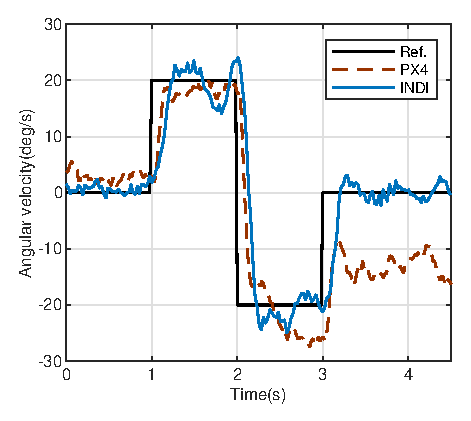
\includegraphics[width=0.48\textwidth]{Fig/Fig8a.eps}%
		\label{Fig:8:a}}\quad   %or \hfil
	\setcounter{subfigure}{3}
	\subfloat[扰动下Roll响应]{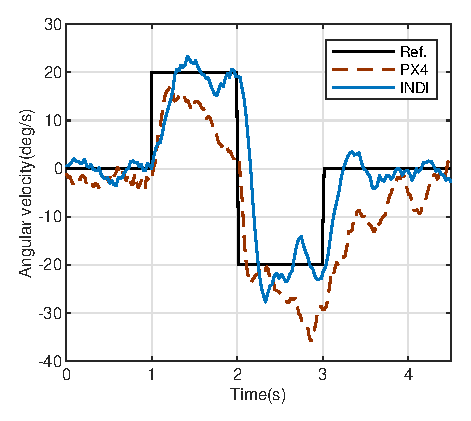
\includegraphics[width=0.48\textwidth]{Fig/Fig8d.eps}%
		\label{Fig:8:d}}\\
	\setcounter{subfigure}{1}
	\subfloat[无扰动下Pitch响应]{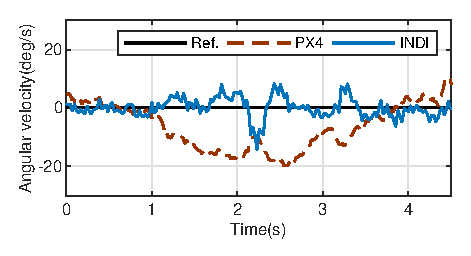
\includegraphics[width=0.48\textwidth]{Fig/Fig8b.eps}%
		\label{Fig:8:b}}\quad
	\setcounter{subfigure}{4}
	\subfloat[扰动下Pitch响应]{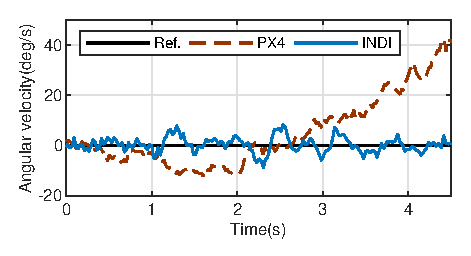
\includegraphics[width=0.48\textwidth]{Fig/Fig8e.eps}%
		\label{Fig:8:e}}\\
	\setcounter{subfigure}{2}
	\subfloat[无扰动下Yaw响应]{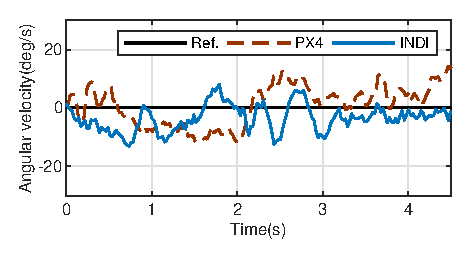
\includegraphics[width=0.48\textwidth]{Fig/Fig8c.eps}%
		\label{Fig:8:c}}\quad
	\setcounter{subfigure}{5}
	\subfloat[扰动下Yaw响应]{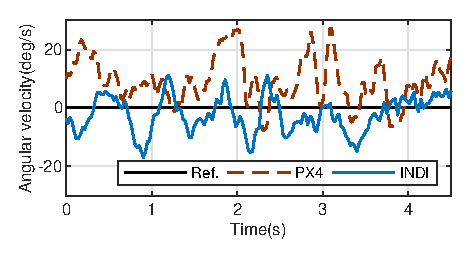
\includegraphics[width=0.48\textwidth]{Fig/Fig8f.eps}%
		\label{Fig:8:f}}
	\caption{\label{Fig:8}试验一结果}
\end{figure}


\section{结论}
在本项工作中,我们提出了一种。


\textbf{\fangsong\xiaosihao 二、过驱动系统的xxxx控制}
\setcounter{section}{0}
\setcounter{subsection}{0}
\section{xxxx控制理论}

\subsection{局部坐标变换}
考虑一个多输入多输出的非线性系统,其形式描述为
\begin{equation}
  \begin{aligned}
    \dot{\bm{x}}&=\bm{f}(\bm{x})+\bm{G}(\bm{x})\bm{u} + \bm{d}(x)\\
    \bm{y}&=\bm{h}(\bm{x})
  \end{aligned}
  \label{system}
\end{equation}

其中,$\bm{f}: \mathbb{R}^{n}\to\mathbb{R}^{n}$ 和 $\bm{h}: \mathbb{R}^{n}\to\mathbb{R}^{p}$ 是光滑的向量场。$\bm{G}$ 是一个光滑函数,将 $\mathbb{R}^{n}\to\mathbb{R}^{n\times m}$ 映射,其中的列是光滑的向量场。$\bm{d}: \mathbb{R}^{n}\to\mathbb{R}^{n}$ 是外部扰动向量。$\bm{y}\in\mathbb{R}^{P}$ 是被控制的输出向量,可以是系统可观测输出的任意子集的函数。当 $p>m$ 时,通过输入输出线性化控制系统是一个欠定问题。当 $p<m$ 时,它变成了超定问题。在大多数有关 INDI 控制的论文中,假设 $p=m$。本文考虑更一般的情况 $p\leq m$。

设 $h$ 的元素为 $h_i, i = 1, 2, ..., p$,矩阵 $G$ 的列向量为 $g_j, j = 1, 2, ..., m$,则 $h_i$ 对向量场 $f$ 和 $g_j$ 的 Lie 导数定义为
\begin{equation}
  \mathcal{L}_{f}h_{i}=\frac{\partial h_{i}}{\partial x}f,\quad\mathcal{L}_{g_{j}}h_{i}=\frac{\partial h_{i}}{\partial x}g_{j},\quad\mathcal{L}_{f}^{k}h_{i}=\frac{\partial(\mathcal{L}_{f}^{k-1}h_{i})}{\partial x}f,\quad\mathcal{L}_{g_{j}}\mathcal{L}_{f}^{k}h_{i}=\frac{\partial(\mathcal{L}_{f}^{k}h_{i})}{\partial x}g_{j}
\end{equation}

如果忽略外部扰动项 $\bm{d}(\bm{x})$,系统 \eqref{system} 的输出动态可以表示为:

\begin{equation}
	\left.\left[\begin{array}{c}y_1^{(\gamma_1)}\\y_2^{(\gamma_2)}\\\vdots\\y_p^{(\gamma_p)}\end{array}\right.\right]=\left[\begin{array}{cccc}\mathcal{L}_f^{\gamma_1}h_1(x)\\\\\mathcal{L}_f^{\gamma_2}h_2(x)\\\vdots\\\mathcal{L}_f^{\gamma_p}h_p(x)\end{array}\right] +  \beta(x)  \boldsymbol{u}
  \end{equation}
  或者
  \begin{equation}
	y^{(\gamma)}=\alpha(x) + \beta(x) \boldsymbol{u}
	\label{outputdynamic}
  \end{equation}
  并且行向量 $dh_{1}(x),\ldots,dL_{f}^{\gamma_{1}-1}h_{1}(x),\ldots,dh_{p}(x),\ldots,dL_{f}^{\gamma_{p}-1}h_{p}(x)$ 是线性无关的。那么系统的相对度 $\gamma$ 满足 $\gamma=\|\gamma\|_{1}=\sum_{i=1}^{p}\gamma_{i}\leq n$,并且 $h_i(x),L_{f}h_i(x),\ldots,L_{f}^{\gamma_{i}-1}h_i(x)$,$1\leq i\leq p$ 可以作为新坐标的一部分。对于 $1\leq i\leq p$,设 
  \begin{equation}
	\begin{aligned}
	  \phi_{1}^{i}(x)&= h_{i}(x)\\
	  \phi_{2}^{i}(x)&= L_{f}h_{i}(x)\\
	  &\vdots\\
	  \phi_{\gamma_{i}}^{i}(x)&= L_{f}^{\gamma_{i}-1}h_{i}(x) 
	\end{aligned}
  \end{equation}
  如果 $\gamma  = n$,对于每个 $\bm{x} \in  \mathbb{D}$,存在一个邻域 $\mathbb{N}$,使得映射 
  \begin{equation}
  \Phi=[\phi_{1}^{1}(x),\ldots,\phi_{\gamma_1}^{1}(x),\ldots,\phi_{1}^{p}(x),\ldots,\phi_{\gamma_{p}}^{p}(x)]^{T}
  \end{equation}
  在 $\mathbb{N}$ 上是一个微分同胚。否则,如果 $\gamma < n$,对于每个 $\bm{x} \in  \mathbb{D}$,总可以找到光滑函数 $\phi_{r+1}(x),\ldots,\phi_{n}(x)$,使得
  \begin{equation}
	\Phi=[\phi_{1}^{1}(x),\ldots,\phi_{\gamma_1}^{1}(x),\ldots,\phi_{1}^{p}(x),\ldots,\phi_{\gamma_{p}}^{p}(x),\phi_{\gamma+1}(x),\ldots,\phi_{n}(x)]^{T}
  \end{equation}
  在 $\bm{x}$ 的邻域 $\mathbb{N}$ 上是一个微分同胚。根据 Frobenius 定理,总是可以选择 $\phi_{r+1}(x),\ldots,\phi_{n}(x)$,使得对所有 $r+1\leq i\leq n$ 和所有 $1\leq j\leq m$,有 $L_{g_{j}}\phi_{i}(x)=0$,对于所有 $x \in \mathbb{N}$。 
  
  总之,如果忽略外部干扰,总可以找到适当的局部坐标变换 $\phi(x)$,在其下,原始系统 \eqref{system} 可以表示为标准形式。设 
  \begin{equation}
	\xi^i=\begin{pmatrix}\xi_1^i\\\xi_2^i\\\vdots\\\xi_{\gamma_i}^i\end{pmatrix}=\begin{pmatrix}\phi_1^i(x)\\\phi_2^i(x)\\\vdots\\\phi_{\gamma_i}^i(x)\end{pmatrix} \quad  
	  \xi=\begin{pmatrix}\xi^1 \\ \vdots \\ \xi^m\end{pmatrix} \quad  
	  \eta=\begin{pmatrix}\eta_1\\\eta_2\\\vdots\\\eta_{n-\gamma}\end{pmatrix}=\begin{pmatrix}\phi_{\gamma+1}(x)\\\phi_{\gamma+2}(x)\\\vdots\\\phi_n(x)\end{pmatrix} \quad   
	  z=\Phi(x)=\begin{pmatrix}\xi\\\eta\end{pmatrix}
	  \label{stran}
  \end{equation}
  然后,方程 \eqref{system} 可以重写为标准形式,为简便起见,我们仍然保留原始坐标,并以向量形式重写系统 \eqref{system} 的标准形式:
  \begin{equation}
	\begin{aligned}&\dot{\eta}= f_{0}(\eta,\xi)\\&\dot{\xi}= A_{c}\xi+B_{c}[\alpha(x)+\beta(x)u]\\&\text{y}= C_{c}\xi\end{aligned}
  \end{equation}
  % \section{增量非线性动态逆的重表述}
  其中 
  \begin{equation}
	A_c=\mathrm{diag}(A_{1},\ldots,A_{m})\quad B_c=\mathrm{diag}(B_{1},\ldots,B_{m})\quad C_c=\mathrm{diag}(C_{1},\ldots,C_{m})
  \end{equation}
  和
  \begin{equation}
	A_i=\left[\begin{array}{ccccc}0&1&0&\dots&0\\0&0&1&\dots&0\\\vdots&&\ddots&&\vdots\\\vdots&&&0&1\\0&\dots&\dots&0&0\end{array}\right]_{\gamma_i \times \gamma_i}, B_i=\left[\begin{array}{c}0\\0\\\vdots\\0\\1\end{array}\right]_{\gamma_i \times 1}, C_i=\left[\begin{array}{ccccc}1&0&\dots&0&0\end{array}\right]_{1 \times \gamma_i}
  \end{equation}
   
  如果考虑外部干扰 $d(x)$,通过坐标变换 \eqref{stran},系统 \eqref{system} 变为 
  \begin{equation}
	\begin{aligned}
	  &\dot{\eta}=\frac{\partial\eta}{\partial x}(f(x)+d(x))\Big|_{x=\Phi^{-1}(z)}= f_{d}(\eta,\xi,d)\\
	  &\dot{\xi}= A_{c}\xi+B_{c}[\alpha(x)+\beta(x)u] + L\\
	  &\text{y}= C_{c}\xi\end{aligned}
	  \label{with_external}
  \end{equation}
  其中
  \begin{equation}
	L=\begin{pmatrix}L^1\\L^2\\\vdots\\L^m\end{pmatrix} \quad \quad \quad L^i=\begin{pmatrix}L_1^i\\L_2^i\\\vdots\\L_{\gamma_i}^i\end{pmatrix}=\begin{pmatrix}L_{d}h_{i}(x)\\L_{d}L_{f}h_{i}(x)\\\vdots\\L_{d}L_{f}^{\gamma_i -1}h_{i}(x)\end{pmatrix} 
  \end{equation}
  INDI 的设计思想是利用输出动态的一阶泰勒展开,在给定动态下解决控制输入的增量。干扰的存在使得系统在新坐标系中的表达相比于标准形式多了一个额外的项 $L$,并且输出动态 $y^{(\gamma)}$ 的表达变得复杂。
  
  \subsection{控制设计}
  在 $t - \Delta t$ 时刻的第一阶泰勒展开为
  \begin{equation}
	\begin{aligned}
	\bm{y}^{(\gamma)}& =\alpha(x)+\beta (x)u + d_y\\
	&=\bm{y}_{0}^{(\gamma)}+\frac{\partial[\alpha(\bm{x})+\mathcal{\beta}(\bm{x})\bm{u}]}{\partial\bm{x}}\Bigg|_{0}\Delta\bm{x}+\mathcal{\beta}(\bm{x}_{0})\Delta\bm{u} + \Delta d_y +O(\Delta\bm{x}^{2})\\
	&=\bm{y}_{0}^{(\gamma)}+\mathcal{\beta}(\bm{x}_{0})\Delta\bm{u}+ \Delta d_y +\delta(z,\Delta t)
	\end{aligned}
  \label{taylor}
  \end{equation}
  其中 $t$ 是当前时刻,下标 0 表示 $t - \Delta t$ 时刻的值。$\Delta x$、$\Delta d_y$ 和 $\Delta u$ 分别表示在一个采样时间步 $\Delta t$ 内的状态、干扰和控制增量。$\delta(z,\Delta t)$ 是展开余项,其表达式为
  \begin{equation}
	\delta(z,\Delta t)=\left[\frac{\partial[\alpha(x)+\beta (x)u]}{\partial x}\Bigg|_{0}\Delta x+O(\Delta x^{2})\right]\Bigg|_{x=\Phi^{-1}(z)}
  \end{equation}
  
  对于像 INDI 或 NDI 这样的反馈线性化方法,核心步骤是提供期望的输出动态 $y^{(\gamma)}$ 并使用输出动态方程求解 $ \Delta u $ 或 $ u $。对于给定的动态 $\bm{y}^{(\gamma)}=\nu_c$,输入增量 $\Delta u=u-u_0$ 通过反转方程 \eqref{taylor} 求解
  \begin{equation}
	\Delta u=\beta ^{-1}(x_{0})(\nu_c-y_{0}^{(\rho)})
	\label{indi}
  \end{equation}
  这被称为 INDI 控制律。
  
  \section{控制分配}
  反演操作的数学本质是求解一个欠定方程,这可以描述为一个控制分配问题:对于给定的 ${{\bm{\nu }}}$,找到 ${{\bm{u }}}\in \Delta $ 使得 ${{\bm{\nu }}}=\bm{\beta}\bm{u}$,或者最小化分配误差 ${{\bm{\nu }}}-\bm{\beta}\bm{u}$,其中 $\Delta $ 是可接受控制的集合,定义为:
  \begin{equation}
  \Delta=\left\{\bm{u} \in \mathbb{R}^{m} \mid u_{min} \leq u_{i} \leq u_{max}, i= 1, 2, ..., m\right\}.
  \label{eq_30}
  \end{equation}
  给定的 ${{\bm{\nu }}}$ 是可达的,如果它包含在可达集(AS)中,记作 $\mathbb{A} $,并定义为:
  \begin{equation}
  \mathbb{A} =\left\{\bm{\nu} \in \mathbb{R}^{p} \mid \bm{\nu}=\bm{\beta} \bm{u}, \bm{u} \in \Delta\right\},
  \label{eq_31}
  \end{equation}
  
  假设 $ \beta $ 具有满行秩,意味着输出动态空间 $ y^{(\gamma)} $ 中的所有向量都可以由 $ u $ 生成。在 INDI 的设计中,假设输入不能产生某些期望的输出动态(例如 $p>m$)是不合理的。此外,在控制分配理论中,通常假设 $B$ 具有鲁棒的满行秩。在实际系统中,可以通过设计有效执行器使其适当定位或通过向实验确定的 $B$ 添加随机扰动来满足这一假设,这超出了本文的范围。总之,我们假设 $B$ 满足鲁棒的满行秩条件。
  
  一个广泛采用的控制分配方法是直接计算 $\bm{\beta}$ 的伪逆:
\begin{equation}
  {{\bm{u }}} = {{\bm{\beta}}^\dag }{{\bm{\nu }}},   \quad  {{\bm{\beta}}^\dag } = {{\bm{\beta}}^T}{\left( {{\bm{\beta}}{{\bm{\beta}}^T}} \right)^{ - 1}}.
  \label{eq_32}
\end{equation}
这种方法称为伪逆方法,它源于无约束的控制分配问题。从优化的角度来看,伪逆方法等价于求解优化问题:对于任何给定的 $\nu$,最小化 $u^T u$,同时满足等式约束 $Bu = \nu$。

然而,当 $u$ 受到约束时,伪逆方法获得的解可能会受到边界条件的限制,即使 $\bm{\nu}$ 保持在其可接受集(AS)内,某些组件的 ${{\bm{\beta}}^\dag }{{\bm{\nu }}}$ 可能会超过其限制,即 ${{\bm{\beta}}^\dag }{{\bm{\nu }}} \notin \Delta$。这导致实际控制效果 $\bm{u}$ 与预期效果 ${{\bm{\beta}}^\dag }{{\bm{\nu }}}$ 不同, 控制分配误差 $\nu - Bu$ 缺乏解析表达式。即使将对 $u$ 的约束纳入等效优化问题,找到 $u$ 的封闭解仍然是困难的。

\subsection{控制量方向保持}
% 另一方面, 
控制量的方向和各通道控制增益有关,它反映了希望控制输入产生的力矩或力的方向,因此有理由认为,实际求解的控制输入$u$是能保持$\nu$的方向是重要的,至少比在输入边界自然截断带来要好。

\subsection{恢复}
上述方法为在$\beta(x)$零空间中寻找控制输入使得满足保方向指标,其解往往倾向于控制边界上的解$u_{da}$。同样,可以在$\beta(x)$零空间移动$u_{da}$,使得$\mathbf{u}=\mathbf{u}_{da}+\mathbf{K}\mathbf{u}^{\perp}$的范数最小,以实现能量最优解。


\section{基于xxxx控制}

在此控制法下的闭环系统动态为
\begin{equation} 
  \begin{aligned}
    &\dot{\eta}= f_{d}(\eta,\xi,d)\\
    &\dot{\xi}= A_{c}\xi+B_{c}[\lambda \nu_c+\Delta d_y+\delta(z,\Delta t) ]\\
    &y= C_{c}\xi
  \end{aligned}
  \label{close}
\end{equation}
\section{稳定性分析}


显然,如果能够估计 $ y_{0}^{(\rho)} $ 并且提高控制频率(即通过缩短时间间隔 $\Delta t$)以改善泰勒展开的近似,INDI 最终能够实现对外部干扰的抑制。设计伪控制 $\nu_c = -K \xi$ 使得 $A_c - B_c K$ 是 Hurwitz的,自然$A_c - B_c \lambda K$也是 Hurwitz的, \eqref{close} 的结果为
\begin{equation}
  \begin{aligned}
    &\dot{\eta}= f_{d}(\eta,\xi,d)\\
    &\dot{\xi}=(A_{c}-B_{c}\lambda K)\xi+B_{c}[\Delta d_y+\delta(z,\Delta t)]
  \end{aligned}
  \label{close2}
\end{equation}
此时分配误差没有显式体现在闭环系统方程中,通过假设 $\Delta d_y+\delta(z,\Delta t)$ 是有界的,并构造适当的 Lyapunov 函数,即可 \eqref{close} 闭环稳定性。证明略。




\textbf{\fangsong\xiaosihao 三、多模态转换}
\setcounter{section}{0}
\setcounter{subsection}{0}
\section{存在问题与研究内容概述}

传统方法在涵道式无人机模型简化与降阶等效上无法达到理想效果,难以实现高效机动轨迹在线规划,极大地制约了涵道式无人机自主机动能力,限制了其潜在应用场景。主要存在以下两个方面的问题:

1)涵道式无人机存在系统气动机理复杂、不确定性高、易受干扰等问题。

2)涵道式无人机具备更强的高超机动能力,而传统的过渡走廊主要针对小动态过程。


本课题拟研究一类涵道式无人机,聚焦于其多模态规划与控制问题。

针对上述涵道式无人机的多模态规划与控制问题,提出一种基于xx的方法框架,目前具体的研究内容包括:


1)涵道无人机非线性动力学特性与系统建模研究。

2)基于xx研究。

最终目标是形成一套基于xx飞行规划与控制方法框架。


\section{系统建模总结}

飞行器动态系统的对象输入为风扇转速$\Omega$,以及舵偏角$\delta_{cv1},\delta_{cv2},\delta_{cv3},\delta_{cv4},\delta_{cv5},\delta_{cv6}$。系统状态为惯性系位置$x^I,y^I,z^I$、惯性系速度$v_x^I,v_y^I,v_z^I$,姿态欧拉角$\varphi,\theta,\psi$,以及角速度$p,q,r$。根据上述工作,可将完整的非线性系统动态方程总结如下:




\section{一般性描述}


上述约束关系与系统模型共同描述了在上述各类假设基础上所有可行系统状态的集合,即为本课题所定义的一般性描述。



\subsection{控制器设计}

针对上述规划轨迹的跟踪问题,底层控制器采用xx结构.


\noindent\rule{1.01\linewidth}{0.3mm}

\section*{与课题相关的学术成果情况:}
\setstretch{1.4} % 设置参考文献行间距,可以按需要调整
% \printbibliography[heading=none]
已录用:xxxx. (xxx2024). 

已投稿:xxxx. (xxx,1区top). 

\end{ubox}


